\documentclass[a4paper,12pt]{article}
\usepackage{amsmath}
\usepackage{bm}
\usepackage[mathscr]{euscript}
\usepackage{graphicx}
\graphicspath{ {images/} }
\begin{document}

\title{Additional Comments on our Code}

\author{Marcel Dürr \and Enes Witwit}

\section{Introduction}

In this document, we will recapitulate our code and provide further explanations on selected excerpts of our code

\section{Mesh}

We start of with our mesh generator 'mesh\_generate'. Our domain $\Omega = [0,1]^2$ will not be subject to change for this task, therefore our only input will be the mesh size $h$. The result will be two matrices, namely \textit{vertex\_matrix} and \textit{cell\_matrix}. \textit{vertex\_matrix} will store the coordinates of each vertex, while \textit{cell\_matrix} only stores the numbers of the four vertices of each cell.
\\
\textit{Example}: $h=0.5$

\[\mbox{\textit{vertex\_matrix}}=\begin{pmatrix} 0&0\\0.5&0\\1&0\\0&0.5\\0.5&0.5\\1&0.5\\0&1\\0.5&1\\1&1\\\end{pmatrix},\ \mbox{\textit{cell\_matrix}}=\begin{pmatrix} 1&2&4&5\\2&3&5&6\\4&5&7&8\\5&6&8&9\\
\end{pmatrix}\]

\section{Shape Functions}

An essential concept for finite element methods would be shape functions. We have to set up certain points, so called \textit{nodes} on a reference cell $\hat T = [0,1]^2$ such that our shape functions $p_i$ are uniquely defined by two properties: 
\begin{enumerate}
\item $p_i(x_j)=\delta_{ij}, \ x_j \mbox{node}$
\item $p_i$ is a polynomial on each edge.
\end{enumerate} 
A way to achieve this, is to choose the location of the nodes in the same way as our mesh. Afterwards, we choose appropriate base-polynomials. If we want polynomials of degree $k$ on the edges, the appropriate basis would be $\{x^iy^j, \ i,j=0...k\}$. Although the resulting polynomials are of order $2k$, they are only of order $k$ in each variable and therefore only of order $k$ on each edge. A mesh generated with mesh-size $\frac{1}{k}$ will yield $k+1$ nodes on each edge; the interpolation is well-posed. \\
\textit{Remark}: The way we order our basis has to be consistent for the entire code, because we only store the coefficients when we want to store a polynomial. In particular, this means that one entry of the coefficient vector must refer to the same polynomial basis element, even for different orders of polynomials. Effectively, this means that the basis for a higher order polynomial can only add basis elements at the end of any lower order polynomial basis. \\
\\
\textit{sf\_generate} follows this scheme closely. Since the shape functions only depend on the polynomial degree $k$ we want to have on the edges, our only input will be the integer $k$. The function will create the nodes using \textit{mesh\_generate} with mesh-size $\frac{1}{k}$. Next, it will create a data-set, containing the coordinates and the value at these coordinates for each node. In total, we get $(k+1)^2:=n$ nodes, their values are computed using the Kronecker Delta. This will ensure, that property 1) holds true when interpolating over all these points. The interpolation is done by solving
\[\begin{pmatrix} 1 &\ x_0 &\ \cdots &\ x_0^ky_0^k \\
\vdots &\ \vdots &\ \ddots &\ \vdots \\ 
1 &\ x_{n} &\ \cdots &\ x_{n}^ky_{n}^k \end{pmatrix}
\begin{pmatrix} a_0 \\ \vdots \\ a_n \end{pmatrix}=\begin{pmatrix} b_0 \\ \vdots \\ b_n \end{pmatrix}\]
The output of our function is the matrix $SF$, which stores the coefficient vectors of each shape function in its rows. Again, we see that a consistent numbering is needed when we want to evaluate a shape function. Let's look at some shape functions:\\
\textit{Example}: Let the polynomial degree on the edges be 1. The four resulting shape functions:\\
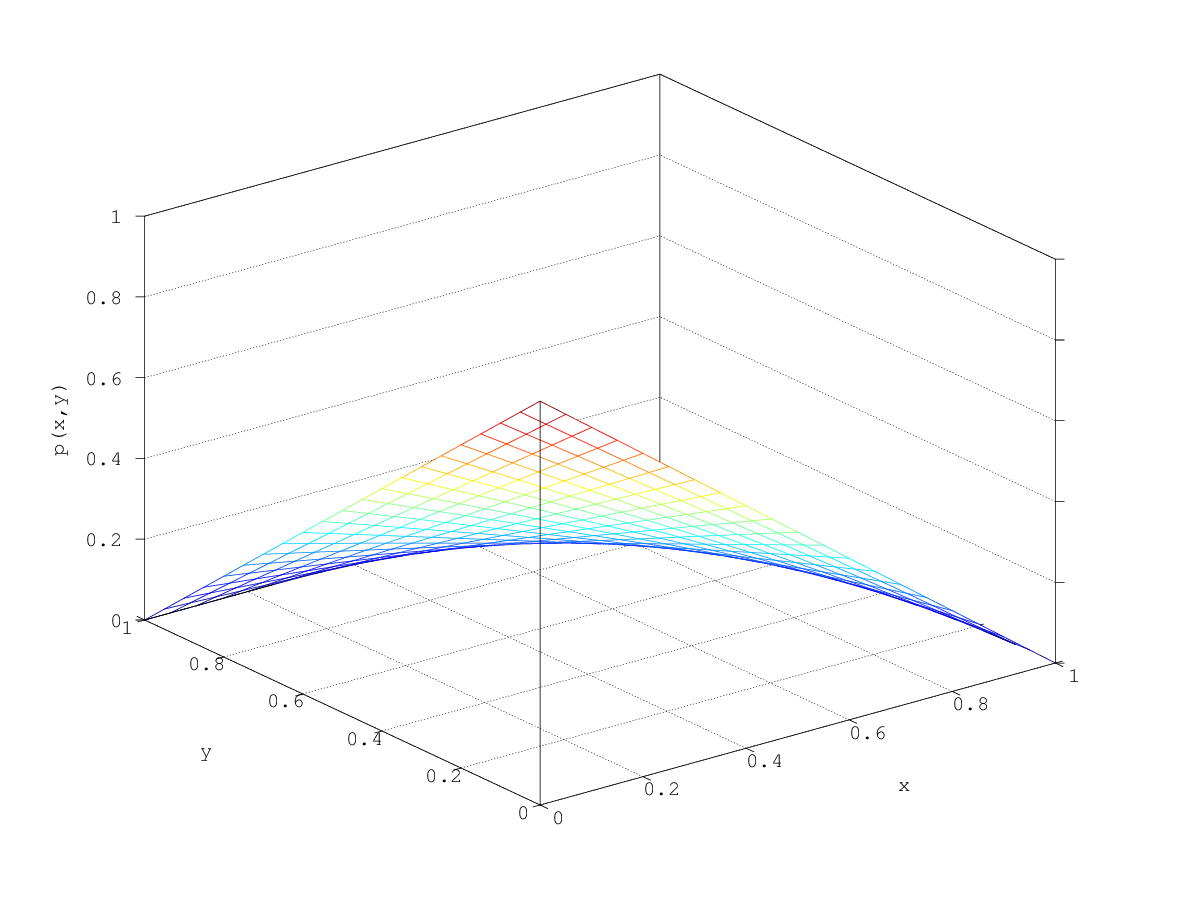
\includegraphics[scale=0.35]{P1} 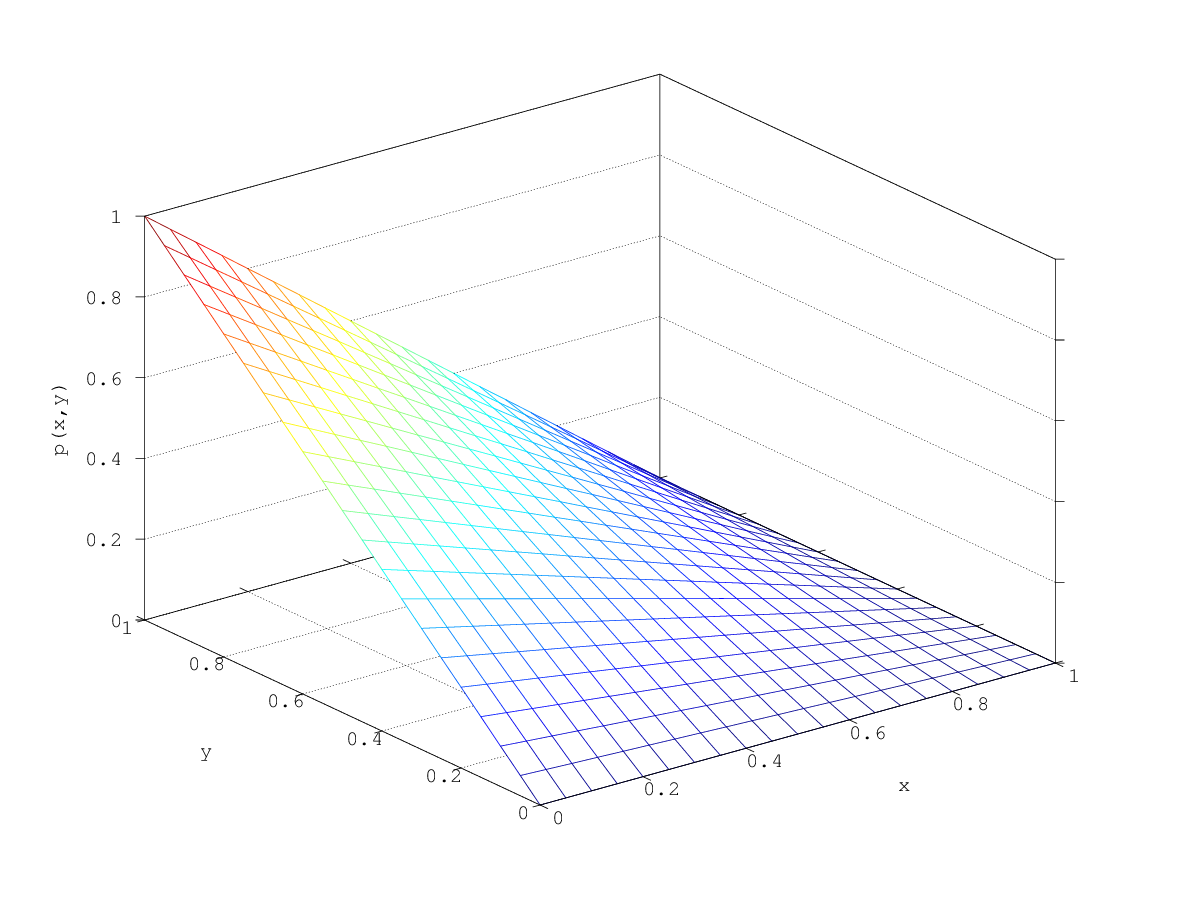
\includegraphics[scale=0.35]{P2} 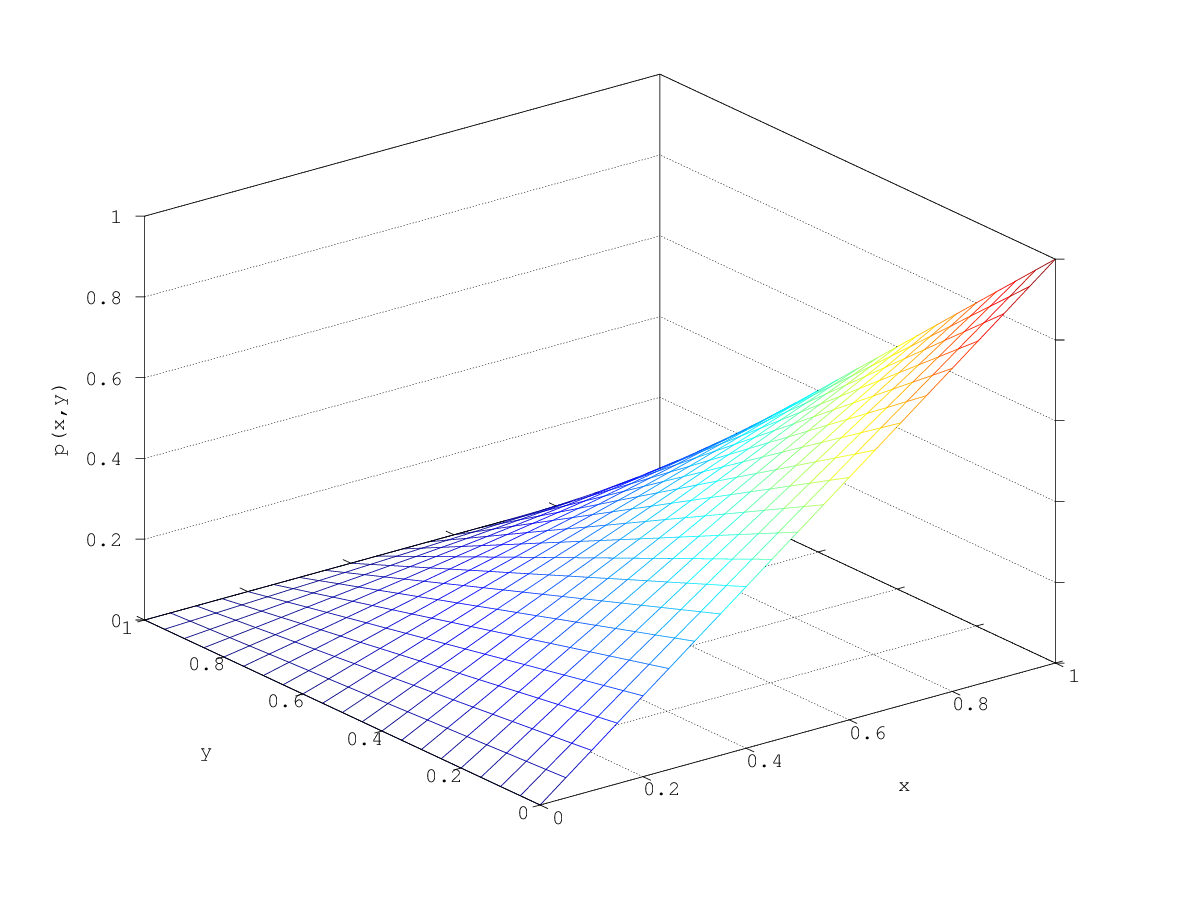
\includegraphics[scale=0.35]{P3} 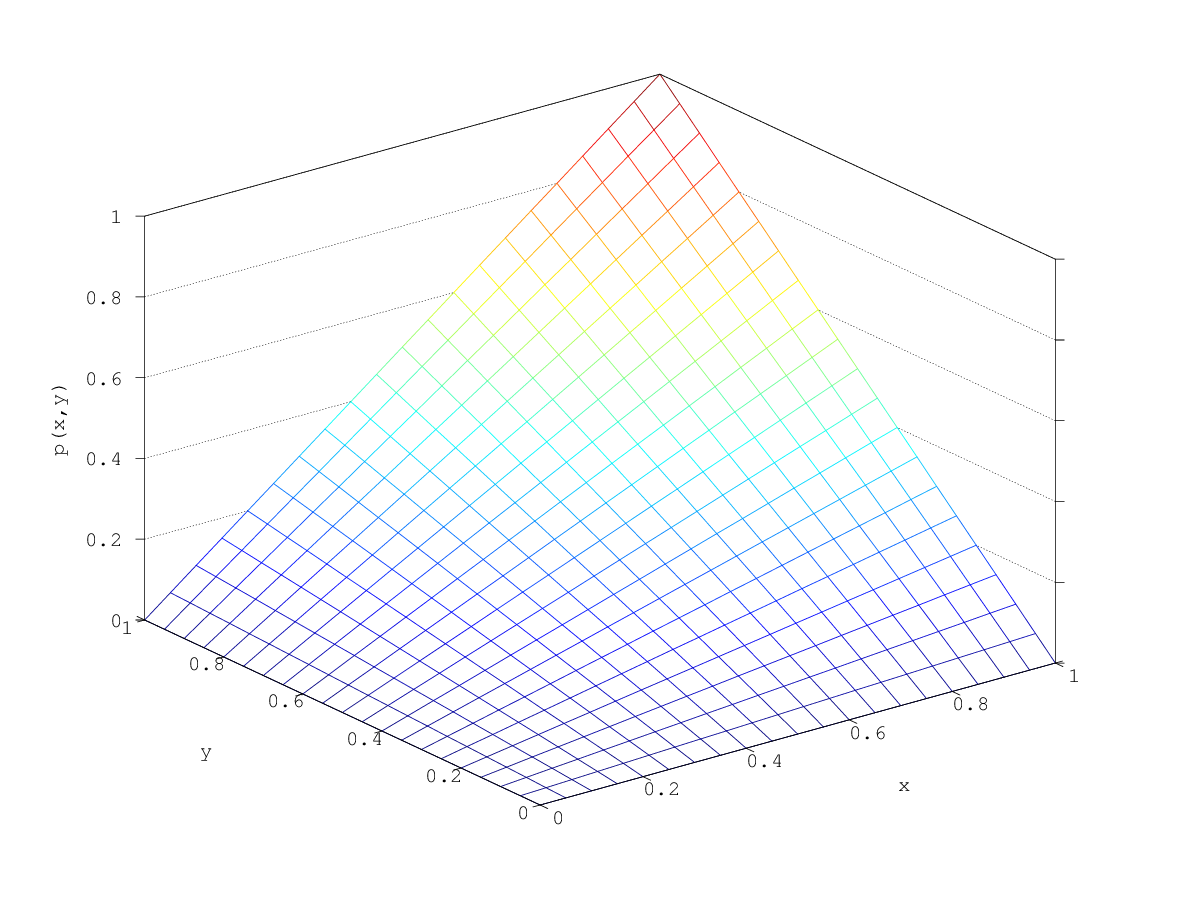
\includegraphics[scale=0.35]{P4}
You can clearly see, that each shape function has the value 1 at one vertex, and 0 at all the other vertices

\section{Stiffness Matrix}
Next up is the assembly of the stiffness matrix, this will be the left hand side of our linear system. The original idea behind the stiffness matrix was to build every combination of our basis functions in our bilinear form, namely $A_{ij}=a(\phi_i,\phi_j)$. As seen in the lecture, it is more efficient to compute a \textit{local} stiffness matrix for each cell, and then insert these values in the right way in a global stiffness matrix. This approach proves to be even more efficient, considering that in our case, the local stiffness matrices are identical for each cell (\textit{see also}: Theoretical Construct, Chapter 'Integrals and Transformations').\\
\\
The computation of the local matrix is done by \textit{sm\_assemble\_local}. As already shown, the computation will not depend on a specific cell, therefore we only need the mesh-size $h$ and the shape function coefficients $SF$. Furthermore, we need several help functions which will compute the required integrals
\begin{itemize}
\item \textit{hf\_eval\_poly} will evaluate a given polynomal at a given point, by using our specific polynomial basis and a coefficient vector
\item \textit{sf\_derivate} will return the coefficient vectors for the derivative in x and y direction for a given polynomial. 
\item \textit{int\_gauss\_weights} will return quadrature points and weigths for a given order and a given quadratic domain.
\item \textit{int\_gauss} will evaluate a given function at the quadrature points and sum over the product of the quadrature weigths. 
\end{itemize} 
Note that the computation of the quadrature points and the actual quadrature is split up into two function. The transformations we use enable us to only integrate over the unit square. Therefore, we only have to compute the quadrature points and weights once. This will save alot of recources.\\
Having these functions at hand, the local matrix can be easily computed. The symmetric bilinear form will result in a symmetric local matrix, we will only compute on half if the matrix.\\
\\
The next step will be the assembly of the global stiffness matrix.

\section{Right Hand Side}
The linear system is still missing its right hand side. We already discussed the computation of it in the 'Theoretical Construct', Chapter 'Integrals and Transformations'. The function \textit{rhs\_integration} will compute the right hand side, it has three essential steps:
\begin{enumerate}
\item Find the cells, on which the current basis function is not vanishing (we will call these cells \textit{active}
\item Find the appropriate shape function for each active cell, to ensure continuity
\item Sum up over all active cells, integrate the appropriate shape functions over the active cell 
\end{enumerate}
The function \textit{node\_to\_cells} will have the number of a global node, the mesh-size and the polynomial degree as an input. It will 'build' a basis function, which has the value $1$ at this node, and $0$ at all the other nodes, by telling us, which shape function we have to evaluate on which cell. Effectively, we will obtain a matrix, with the cell number in one column, and the appropriate shape function number in the other column. Step 1) and 2) are therefore done.\\
\\
Step 3) will only consist of the computation of the integrals, which will be handled by our functions \textit{int\_gauss} and \textit{int\_gauss\_weights}. We will use the transformations we already discussed in the chapter 'Integrals and Transformations'.

\section{Linear Solvers}
The global stiffness matrix will be sparse, due to the way we chose the basis functions (zero on the vast majority of the cells). The prefered solvers for linear systems with sparse matrices are iterative solvers. We implemented two common algorithms, namely the \textit{generalized minimal residual method} and the \textit{conjugate gradient method}. 
We are left with a coefficient vector $u$. We will get our solution, by building the linear combination of the basis ${\phi_i}$ with $u$: 
\[u_h = \sum \phi_i u_i\]
Remember, that we do not actually have the basis functions $\phi_i$ at hand, since we accessed the needed values by using shape functions and transforming the integral. We will need an auxiliary function to evaluate $u_h$

\section{Evaluation of the Solution}
The idea behind \textit{hf\_eval\_solution} is to find the indices of the basis functions, that do not vanish at a given point $(x,y)$. Similar to the calculation of the right hand side, we will need to know which shape function should be evaluated at which cell. Additionally, we need to know to which entry of the coefficient vector $u$ the computation correlates.\\
\textit{hf\_eval\_solution} starts off by searching for adjacent cells to the given point $(x,y)$, at which we want to evaluate our solution. Once we have the numbers of the active cells, we want to know, which nodes are located on these cells. We do know, that for every node in one of the active cells, we get a non-zero basis function at $(x,y)$, with a correlating entry in $u$.  



In order to apply some of the results from the lecture, we need to derive the weak formulation of the given problem 
\begin{align}
\mbox{Find } u\in C^2(\Omega)\mbox{ :}-\Delta u+u &= \cos(\pi x)\cos(\pi y) &&\mbox{in } \Omega \\
\partial _n u &= 0 &&\mbox{on } \partial\Omega.
\end{align}
Multiplying with an arbitary $v\in C^2(\Omega)$ and integrating over $\Omega$ gives us
\[-\int _\Omega \Delta uv \,\mbox{d} \bm{x} + \int _\Omega uv \,\mbox{d} \bm{x} = \int _ \Omega fv\,\mbox{d} \bm{x}\]
where $f=\cos(\pi x)\cos(\pi y)$ and $\bm{x}=(x,y)$. Using Green's first formula and (2) we can obtain the weak formulation
\[\int _\Omega \nabla u\nabla v \,\mbox{d} \bm{x} + \int _\Omega uv \,\mbox{d} \bm{x} = \int _ \Omega fv\,\mbox{d} \bm{x}\]
From now on, we will denote the left hand side of the equation by $a(u,v)$ and the right hand side by $F(v)$. Thus, we obtain the weak formulation
\begin{equation}
\mbox{Find }u\in H^1(\Omega) \mbox{ :} \quad a(u,v)=F(v)\quad \forall v \in H^1(\Omega)
\end{equation}

\section{Existence and Uniqueness of a Solution}

We can already see, that our bilinear form $a(\cdotp ,\cdot)$ is the inner product associated with the norm on our function space $H^1(\Omega)$. We want to use the Riesz representation theorem to prove existence and uniqueness of a solution. In order to do so, it remains to show that our functional $F(\cdot)$ is linear and bounded. Linearity follows from the properties of integration. Using Hoelder's inequality, we show that
\begin{align*}
F(u)&=\|fu\|_{L^1(\Omega)}\\
	&\stackrel{\tiny\mbox{Hld.}}{\le} \|f\|_{L^2(\Omega)}\|u\|_{L^2(\Omega)}\\
	&\le \|1\|_{L^2(\Omega)}\ \big(\|u\|_{L^2(\Omega)}+\|u\|_{L^2(\Omega)}\big)\\
	&\le c\ \|u\|_{H^1(\Omega)}\mbox{,}
\end{align*}
where c depends on our domain $\Omega$. For our case, we have $\Omega=[0,1]^2$, in particular this means that $\Omega$ is bounded and our constant $c$ is finite. Therefore, $F(\cdot)$ is a bounded, linear functional and we can apply the Riesz representation theorem.

\section{Finding the Analytical Solution}

Now that we know that a unique solution exists, we want to actually compute it. We will use the ansatz $u=C\cos(\pi x)\cos(\pi y)$, with its gradient $\Delta u=2\pi^2 u$. Inserting in (1) gives us
\begin{equation}
-2C\pi^2 \cos(\pi x)\cos(\pi y) + C\cos(\pi x)\cos(\pi y)=\cos(\pi x)\cos(\pi y)
\end{equation}
\begin{align}
&\Rightarrow - 2C\pi^2 + C =1\\
&\Leftrightarrow C = \frac{1}{1-2\pi^2}
\end{align}
This leaves us with the solution $u=\frac{1}{1-2\pi^2}\cos(\pi x)\cos(\pi y)$.

\section{Integrals and Transformations}

The transformations we have to use for our FEM-code are very simple, since our mesh will be generated uniformly. Ultimately, we will only have to scale and displace our reference cell. We decided, that we will hard-code this property, since it will heavily simplifiy the computation of the local stiffness-matrices and the right-hand-side of the linear system, as we will see in brief.
\\ \\
Let $T$ be a cell of the mesh with vertices $v_1,v_2,v_3,v_4$, where $v_1$ is the vertex on the bottom left and h is the length of every edge. $\hat T = [0,1]^2$ shall be our reference cell. Then, our transformation $F$ will look like 
\[F \smash : \  \hat T \rightarrow T, \ \ \bm{\hat x}=\begin{pmatrix}\hat x \\ \hat y \end{pmatrix} \mapsto \begin{pmatrix}h \ 0 \\ 0 \ h\end{pmatrix} \begin{pmatrix}\hat x \\ \hat y \end{pmatrix} + v_1 := \begin{pmatrix}x\\y\end{pmatrix} := \bm{x}\]
We immediately can see, that the jacobian $J$ is given by
\begin{equation}
J(\bm{\hat x})=J=\begin{pmatrix}h \ 0\\0 \ h\end{pmatrix}\mbox{,}
\end{equation}
in particular, it is independet of $\bm{\hat x}$. Consequently, we also get
\begin{equation}
|\mbox{det}(J(\bm{\hat x}))|=|\mbox{det}(J)|=h^2\mbox{and} \ J^{-1}=h^{-1}\begin{pmatrix}1 \ 0 \\ 0 \ 1\end{pmatrix}
\end{equation}
Using the results from the lecture on the transformation of our bilinear form $a(\cdotp, \cdot)$ and using (7) and (8), we can compute the stiffness matrix in the following way
\[a^{(T)}_{ij} = \int_{\hat T}\nabla p_i \,\cdotp \nabla p_j\,\mbox{d}\bm{\hat x} + h^2\int_{\hat T}p_i p_j\,\mbox{d}\bm{\hat x}\mbox{,}\]
where $p_i$ and $p_j$ are our shape functions.\\ \\
\textit{Remark:} Note that the $\nabla$ in our formula refers to the gradient with respect to $\bm{\hat x}=\begin{pmatrix} \hat x \\ \hat y\end{pmatrix}$.
\textit{Remark:} Note that for affine transformations, the local stiffness matrices do not depend on the cell $T$, for which we want to compute it. Therefore, every local matrix looks the same and we only have to compute it once.
\\ \\
For the right-hand side, we have to look at the substitution formula for higher dimension integrals. But first of all, we need do split the intagral up. Let $\phi_i$ be a basis function of our domain $\Omega$, $\mathscr{T}_h$ our meshcells and $\mathscr{T}_i$ the mesh cells, on which $\phi_i \neq 0$. Then we get
\begin{align*}
\int_{\Omega}f(\bm{x})\phi_i(\bm{x})\ \mbox{d}\bm{x}&=\sum_{T\in\mathscr{T}_h} \int_Tf(\bm{x})\phi_i(\bm{x})\ \mbox{d}\bm{x} \\
													&=\sum_{T\in\mathscr{T}_i} \int_Tf(\bm{x})\phi_i(\bm{x})\ \mbox{d}\bm{x} \\
													&=\sum_{T\in\mathscr{T}_i} \int_Tf(\bm{x})p^{(T)}_{i^{(T)}}(\bm{x})\ \mbox{d}\bm{x} \\
													&=\sum_{T\in\mathscr{T}_i} \int_{\hat T}f(F^{(T)}(\bm{\hat x})\hat p_{i^{(T)}}(\bm{\hat x})|\mbox{det}(J)|\ \mbox{d}\bm{\hat x} \\
													&=h^2\sum_{T\in\mathscr{T}_i} \int_{\hat T}f(h\bm{\hat x}+v^{(T)}_1)\hat p_{i^{(T)}}(\bm{\hat x})\ \mbox{d}\bm{\hat x}						
\end{align*}

\end{document}
